\section{Redox-Reaktionen}
Redox-Reaktionen sind Elektronenübertragungs-Reaktionen. Dabei findet gleichzeitig eine Reduktion und eine Oxidation statt.

\subsection{Oxidation und Reduktion}
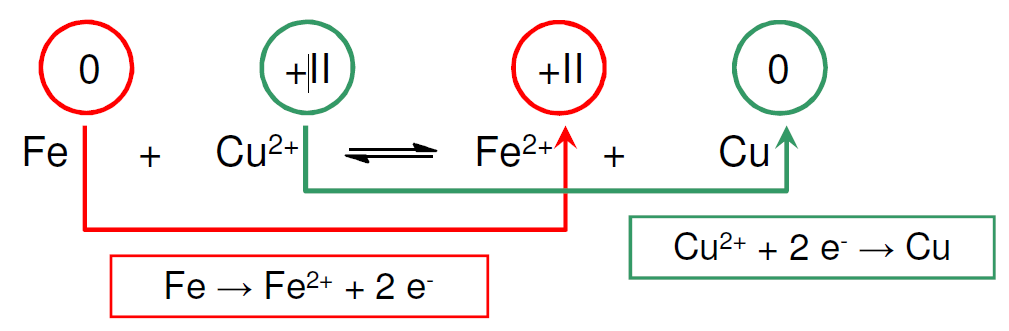
\includegraphics[width=0.6\linewidth]{images/9_Redox_Reaktion.png}\\
Oxidation (rot) = Elektronenabgabe, $X^m \Rightarrow X^{m+1} + e{^-}$\\
Bei der Oxidation wird die Oxidationszahl erhöht. Ein Reduktionsmittel (Elektronenspender) gibt Elektronen ab, dabei wird es oxidiert, es wird zum Oxidationsmittel (Elektronenakzeptor).\\

Reduktion (grün) = Elektronenaufnahme, $Y^n + e{^-} \Rightarrow Y^{n-1}$\\
Bei der Reduktion wird die Oxidationszahl reduziert. Ein Oxidationsmittel nimmt Elektronen auf, dabei wird es reduziert, es wird zum Reduktionsmittel.\\

\subsection{Oxidationszahlen (OZ)}
Um eine Redox-Reaktion erkennen zu können, muss man wissen, welcher Stoff $e^-$ aufnimmt (oxidieren) bzw. $e^-$ abgibt (reduzieren). Oxidationszahlen werden mit römischen Ziffern geschrieben. \\
Zur Bestimmung der OZ gelten folgende Regeln:
\begin{enumerate}
	\item Die OZ der Atome in ihrer elementaren Form ist 0, Bsp. $O_2^0$, $Na^0$
	\item Bei einatomigen Ionen entspricht die OZ der Ionenladung (siehe Salze), Bsp. $Na^+$: OZ=+I
	\item Bei Molekülen werden die Bindungselektronen dem elektronegativeren Atom zugeordnet. 
	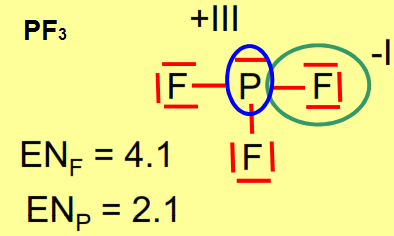
\includegraphics[width=4cm]{images/RedoxRegel3.png}\\
	Faustregeln: $F$ immer -I, $O$ fast immer -II, $H$ fast immer +I
	\item Die Summe aller OZ muss der Ladung des Teilchens entsprechen. Bsp: $H_3O^+$\\
	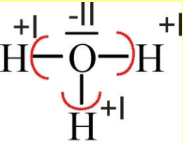
\includegraphics[width=2cm]{images/RedoxRegel4.png}
\end{enumerate}

\subsection{Vorhersage Brennbarkeit eines Stoffes}
Verbrennunsreaktionen sind Reaktionen mit Sauerstoff $O_2$. Dabei wirkt $O_2$ als Oxidationsmittel. Ein Stoff ist theoretisch brennbar, wenn er Elemente enthält, die noch nicht in der (für das jeweilige Element) höchsten Oxidationsstufe vorliegen. Dies kann man wie folgt prüfen:
\begin{enumerate}
\item Oxidationszahlen mittels obigen Regeln bestimmen.
\item Prüfen ob bereits die höchste Oxidationsstufe eines Stoffes vorliegt (Abgleich mit PSE $\Rightarrow$ höchste positive Oxidationszahl). Falls ja, nicht brennbar, sonst brennbar!
\end{enumerate}

\subsection{Die Redox-Reihe}
Die Redox-Reihe gibt Auskunft über die Stärke eines Stoffs als Reduktions- bzw. Oxidationsmittels. Eine Redox-Reaktion kann ablaufen, wenn das Reduktionsmittel höher in der Tabelle liegt als das Oxidationsmittel.\\

Tabelle siehe Anhang. \\

\subsection{Das Redox-Potential}
Das Redox-Potential beschreibt das Reduktions- bzw. Oxidationsvermögen einer Halbzelle (Redoxpaar) in Volt. In der Redox-Reihe ist für jedes Redoxpaar ein Standard-Redox-Potential (1 mol/l, 1013 mbar, 25$^\circ$C) aufgeführt. Redoxpaare mit einem hohen Elektronendruck sthen in der Redox-Reihe weit oben, sie haben ein negatives Redox-Potential. Umgekehrtes gilt für Paare mit einem tiefen Elektronendruck.\\

\subsubsection{Edle und unedle Metalle}
\emph{Edle} Metalle: $E^0 > 0V$, zeigen kaum Reaktion mit $O_2, H_2O$, Säuren. Kommen gediegen in der Natur vor. \\
\emph{Unedle} Metalle: $E^0 < 0V$, gehen mit vielen Stoffen Reaktionen ein. Kommen in der Natur nur in Form von Verbindungen vor. \\

\subsubsection{Konzentrationsabhängigkeit des Redox-Potential}
Das Standard-Potential $E^0$ einer Halbzelle ist definiert für eine Ionen-Konzentration von 1 mol/l. Das effektive Redoxpotential wird gemäss der \emph{Nernst}-Gleichung beschrieben:
\begin{eqnarray*}
	E_{RM/OM} &= E^0_{RM/OM} + \frac{R \cdot T}{z \cdot F} \cdot \ln\frac{[OM]}{[RM]} \\ &=  E^0_{RM/OM} + \frac{0.059V}{z} \cdot \lg\frac{[OM]}{[RM]}
\end{eqnarray*}
mit der Gaskonstante $R=8.214\frac{J}{mol \cdot K}$, der Temperatur $T$ in $K$, der Faraday-Konstante $F=96485\frac{C}{mol}$ und der Zahl der übertragenen Elektronen pro Formeleinheit $z$ (aus Redox-Reihe). Zudem gilt, für feste Metalle (und andere unlösliche Stoffe) ist [RM] konstant und wird in der Nernstschen Gleichung = 1 gesetzt. \\

Generell: je kleiner die Konzentration, desto unedler das Redox-Potential.

\subsubsection{Die pH-Abhängigkeit des Redox-Potential}
Sind an einem Redoxpaar auch Protonen ($H^+$) beteiligt, so ist das Redox-Potential auch vom pH-Wert abhängig.\\\\
Redoxpaar $H_2 + 2 H_2O$ \& $2 H_3O^+ + 2 e^-$: \\ $E = -0.059V \cdot pH$ \\
Redoxpaar $4 OH^-$ \& $O_2 + 2 H_2O + 4 e^-$: \\ $E = 1.23 - 0.056V \cdot pH$ \\

Generell: je saurer (tiefer) der pH-Wert, desto edler das Redoxpotential. \\


